%-------------------------------------------------------------------------------
% Preamble
%-------------------------------------------------------------------------------

\documentclass[twocol]{ametsoc}
\journal{mwr}

%Citations should be of the form ``author year''  not ``author, year''
\bibpunct{(}{)}{;}{a}{}{,}

%Packages
\usepackage{
	siunitx, % units
	cleveref,% cross-references
	physics, % better physics notation
	url, % for URLs
	amsmath, % for math
	array, % for fixed-width tables
}
\newcolumntype{L}[1]{>{\raggedright\let\newline\\\arraybackslash\hspace{0pt}}m{#1}}


%-------------------------------------------------------------------------------
% Title and Authors
%-------------------------------------------------------------------------------

\title{Extreme rainfall in Paraguay during the 2015-2016 austral summer: causes and subseasonal-to-seasonal predictive skill}
\authors{James Doss-Gollin\correspondingauthor{James Doss-Gollin. Dept. of Earth and Environmental Engineering, Columbia University, 500 W. 120th St., New York, NY. USA.}}
\affiliation{Dept. of Earth and Environmental Engineering, Columbia University, 500 W. 120th St., New York, NY. USA \\ Columbia Water Center, Columbia University, 500 W. 120th St., New York, NY. USA}
\email{james.doss-gollin@columbia.edu}
\extraauthor{\'Angel G. Mu\~noz}
\extraaffil{Atmospheric and Oceanic Sciences (AOS). Princeton University. Princeton, NJ 08540-6649. USA  \\
	International Research Institute for Climate and Society (IRI). The Earth Institute. Columbia University. Palisades, NY. 10964-1000. USA}
    \extraauthor{Simon J. Mason}
\extraaffil{International Research Institute for Climate and Society (IRI). The Earth Institute. Columbia University. Palisades, NY. 10964-1000. USA}
\extraauthor{Max Past\'{e}n}
\extraaffil{Direcci\'{o}n de Meteorolog\'{i}a e Hidrolog\'{i}a. Paraguay \\
	Facultad Polit\'ecnica. Universidad Nacional de Asunci\'{o}n. Paraguay}


%-------------------------------------------------------------------------------
% Abstract
% Up to 250 words in length
%-------------------------------------------------------------------------------

\abstract{
	During the austral summer 2015-16 severe flooding displaced over 150,000 people on the Paraguay River system in Paraguay, Argentina, and Southern Brazil. This flooding was out of phase with the typical seasonal cycle of the Paraguay River, and was driven by repeated intense rainfall events in the Lower Paraguay River basin. Using a weather typing approach within a diagnostic framework, we show that enhanced moisture inflow from the South American Low-Level Jet, and local convergence associated with baroclinic systems favored the development of mesoscale convective activity and enhanced precipitation. The observed circulation patterns were made more likely by the cross-timescale interactions of multiple climate modes, including a very strong, mature El Ni\~no event and an unusually persistent Madden-Julian Oscillation in phases four and five.
	The rainfall skill is assessed using seasonal forecasts produced by the Latin American Observatory of Climate Events (OLE2), and sub-seasonal forecasts produced by the European Centre for Medium-Range Weather Forecasts. The probabilistic seasonal forecasts accurately predicted above-normal rainfall over the region. Although raw sub-seasonal forecasts exhibited limited skill at lead times beyond the first predicted week (i.e., week 1), it is found that a Model Output Statistics approach involving principal component regression substantially improves skill for week 3, being also better than other bias-correction methods based on canonical correlation analysis and extended logistic regression. Possible implications for flood preparedness are briefly discussed.
}

\begin{document}

%% Necessary!
\maketitle

%-------------------------------------------------------------------------------
% Introduction
%-------------------------------------------------------------------------------

\section{Introduction}

% THIS PARAGRAPH NEEDS SOME WORK
% COME BACK TO IT LATER
During the austral summer of 2015-16, repeated intense rainfall events led to severe flooding on the Paraguay River, displacing approximately \num{170000} people \citep{BrackenridgeDFO} and generating tremendous property damage.
The Paraguay River (\cref{fig:study-area}) is the primary tributary of the Paran\'{a} River and an important contributor to the La Plata basin, and its flooding directly impacts the Paraguayan cities of Asunci\'{o}n, Concepci\'{o}n, and Pilar, and the Argentine cities of Formosa and Corrientes.
Intense rainfall and flooding along the Paraguay River also has important implications for hydropower generation along the Paran\'{a} River, for agriculture, and for regional water resource management.
Until now, the drivers of the November-February (NDJF) 2015-16 rainfall events and the extent to which they could have been skilfully predicted has not been analyzed in the scientific literature.
The goal of this paper is to address these issues.

% Climatology and past floods
The rainfall climatology of the Paraguay River basin varies strongly by season, with extratropical characteristics in the winter and monsoonal characteristics in the summer.
In the summer season (NDJF), the focus of this study, circulation is dominated by the upper-tropospheric Bolivian High, the lower-level subtropical highs, the Chaco Low over northern Argentina, the South Atlantic Convergence Zone (SACZ), and the South American Low-Level Jet, or SALLJ \citep{Grimm2009,Marengo:2012cm}.
Rainfall in the Lower Paraguay River Basin peaks around \SI{5}{\milli\meter\per\day} during the warm months (October-May) and reaches a minimum near \SI{2}{\milli\meter\per\day} in July and August.
However, the flat topography limits the ability to carry the summer runoff, causing seasonal innundation of the Pantanal and distributing the river discharge in time \citep{Bravo:2011et,Barros:2004bn}.
Thus, the streamflow maxima typically occurs in phase with precipitation upstream of the Pantanal, while downstream of the Pantanal -- over the Lower Paraguay River -- the annual peak, including for extreme flood events, typically occurs between April and July \citep{Barros:2004bn}.

% SALLJ and MCS
A large fraction of rainfall, and nearly all intense rainfall, in the Paraguay River Basin during the summer is associated with mesoscale convection \citep{Velasco1987}.
Previous studies of organized convection and precipitation across subtropical continental South America have found close correspondence to the exit region of the low-level jets \citep{Saulo:2007km,Salio:2007gd,Marengo2004,Velasco1987}, which is influenced in both summer and winter by midlatitude baroclinic wave trains that interact with the Andes topography to generate orographically bound cyclones and northerly low-level flow \citep{Campetella:2002hx,Seluchi:2006bi,Boers:2014gt}.
The strength and direction of this moisture transport varies substantially between events; SALLJ exit regions range from central Argentina \citep[``Chaco Jet Events'';][]{Salio:2002ev} to southeastern Brazil. In addition, the relationship between the low-level jet and convection involves two-way feedback \citep{Saulo:2007km}.

% S2S Drivers
At sub-seasonal timescales, convection in the Paraguay River Basin is modulated by a variety of drivers, notably including the SACZ and the Madden-Julien Oscillation (MJO).
During SACZ (NoSACZ) conditions, strong (weak) convergence is observed over the Amazon basin with divergence (convergence) over southwestern Brazil, northern Argentina and Paraguay \citep{Herdies:2002jy,Carvalho2010}.
SACZ occurrence is related to westerly wind regimes, as well as ``active'' and ``break'' periods of the South American Monsoon \citep{Marengo2004}.
\citet{Carvalho2004} and \citet{Jones2002} demonstrate that mid-latitude dynamics influence low-level wind anomalies on many time scales, but also find that tropical-extratropical interactions complicate attempts to find one-way casual relationships.

% Seasonal Drivers
At seasonal timescales, El Ni\~no-Southern Oscillation (ENSO) is the dominant driver of convection variability in the Paraguay River Basin.
During El Ni\~no years, a low-level anticyclonic anomaly over central Brazil enhances occurrence of the low-level jet, favoring the development of mesoscale convective systems \citep{Velasco1987}.
The impact of ENSO events is felt partly by changes in the SACZ, which change due to ENSO-induced extratropical Rossby wave trains \citep{Grimm:2011vp}.
There is also intraseasonal variability of rainfall during El Ni\~no years, typically including a reversal between November and January of the following year, which are likely dominated by land-surface interactions \citep[see][]{Grimm2009,Grimm2003}.
These findings suggest that while interannual variability during the spring may be driven by remote processes,  during the summer local processes dominate.
In particular, regional land-surface feedbacks can cause regions that exhibit wet anomalies in the spring to experience, on average, more summer precipitation \citep{Grimm:2009bq}.

The paper continues as follows.
In \cref{sec:data} we describe our data sources, while in \cref{sec:methods} we provide an overview of technical methods carried out.
In \cref{sec:diag} we diagnose the circulation patterns associated with intense rainfall during NDJF 2015-16, using composite and weather typing approaches.
In \cref{sec:fcsts} we examine forecasts of rainfall in the Lower Paraguay River Basin and assess forecast skill, with special attention to the first week of December, when the most important flooding events started.
In \cref{sec:discussion} we discuss potential implications of our findings and potential future work.
Finally, in \cref{sec:summary} we summarize our results.

%-------------------------------------------------------------------------------
% DATA
%-------------------------------------------------------------------------------

\section{Data} \label{sec:data}

The analysis involves observations and model forecasts.

\subsection{Observations}

The period analyzed for diagnostics purposes is from 01 Nov 1979 through 29 Feb 2016.

Rainfall data is taken from the CPC Unified Gauge-based Analysis of Global Daily Precipitation dataset \citep{xie2010cpc}, available online at \url{http://iridl.ldeo.columbia.edu/SOURCES/.NOAA/.NCEP/.CPC/.UNIFIED_PRCP/.GAUGE_BASED/.GLOBAL/.v1p0/}.
Spatial resolution is \SI{0.5}{\degree}, and temporal resolution is daily.
Both the retro and real-time datasets are used.

Atmospheric circulations are diagnosed using daily data from the NCAR-NCEP Reanalysis I data set \citep{Kalnay1996}, available online at \url{https://www.esrl.noaa.gov/psd/thredds/dodsC/Datasets/ncep.reanalysis/}.
Spatial resolution is \SI{2.5}{\degree}, which is adequate for synoptic-scale analyses.

Because the end-of-day time for the rainfall data is 12:00GMT over most of South America, we use six-hour reanalysis data, and shift by twelve hours before re-sampling to the daily time step.
This ensures that the time steps in the reanalysis and rainfall data sets are the same, but means that a day is defined as beginning at 12:00 GMT.
Since most summer rainfall in this region occurs overnight, this end-of-day time (which translates to approximately 8:00 AM locally depending on the exact time zone) tends to separate distinct events.

Streamflow data was collected by the Paraguayan Navy and National Administration of Navigation and Ports of Paraguay, and was processed and distributed by the Paraguayan Directorate of Meteorology and Hydrology (DINAC-DMH).
Locations of streamflow gauges are shown in \cref{fig:study-area}.

\subsection{Climate Indices}

This study also makes use of some climate indices.
Data on the El Ni\~{n}o-Southern Oscillation (ENSO) came from a statistical-dynamical interpolation \citep{Kaplan:1998df}, which is constrained by relatively high-quality observations during the study period and is available online at \url{http://iridl.ldeo.columbia.edu/SOURCES/.Indices/.nino/.EXTENDED/.NINO34/}.
Data on the Madden-Julien Oscillation (MJO) came from the Australian Bureau of Meteorology and is available online at \url{http://www.bom.gov.au/climate/mjo/graphics/rmm.74toRealtime.txt}.


\subsection{Model forecasts}



This study analyzes probabilistic seasonal and sub-seasonal forecasts of extremely wet rainfall events, defined in the same way as in observations (90th percentile).

The sub-seasonal forecasts used were isseud by the European Centre for Medium-Range Weather Forecasts (ECMWF) using a coupled model, available via the Subseasonal-to-Seasonal Prediction Project Database \citep{Vitart2016}.
The horizontal resolution is \SI{1.5}{\degree} deg.
Forecasts consider the period starting in Dec 2015 until Mar 2016 and hindcasts to assess the real-time predictive skill consider the period Dec 1-7, 1995-2014.
There is a total of 51 ensemble members for each forecast, and 11 ensemble members for each one of the 20 hindcasts (Dec 1-7, 1995-2014).

Hindcasts were used to define the extreme event threshold, and for probabilistic forecast verification; forecasts were used to analyze modeled rainfall during the entire NDJF 2015-16 season and in particular the week of Dec 1-7, 2015.
For probabilistic analysis of the rainfall during the week 1-7 December 2015, rainfall forecasts and hindcasts considered were initialized on November 12th and 16th, 2015.
For plotting, all forecast initializations were considered.
These steps are discussed further in subsequent sections.

The seasonal predictions used were ``flexible format'' forecasts provided by the International Research Institute for Climate and Society (IRI).
This product provides the probability of exceedance (or non-exceedance) of a user-specified percentile of the climatological distribution.
The DJF 2015-2016 forecasts analyzed were produced in November 2015.
Due to the short record of flexible format forecasts (2012-2016), no verification was performed for seasonal predictions.
These forecasts are provided at a horizontal resolution of \SI{2.5}{\degree}.


%-------------------------------------------------------------------------------
% METHODS
%-------------------------------------------------------------------------------

\section{Methods} \label{sec:methods}

Different types of analyses are used to diagnose the causes of the extreme rainfall events, and to bias-correct and verify the forecasts.
All codes used for data and analyis are available at \url{https://github.com/jdossgollin/PYFloods}.
Computation with multidimensional data was performed using the \texttt{xarray} \citep{hoyer2017xarray} and \texttt{numpy} \citep{vanderWalt:2011dp} packages of the python computing environment; computations on tabular data utilized the \texttt{pandas} \citep{McKinney:2010un} package; and plotting was performed with the \texttt{matplotlib} \citep{Hunter:2007ux} and \texttt{cartopy} \citep{Cartopy} packages.

\subsection{Climatology and Anomalies} \label{sec:climatology-anomalies}

The climatological value of a field (rainfall or a circulation variable from reanalysis) is defined as the mean, at each grid cell, during the period $\qty[1980, 2010]$.
The anomaly, for a particular date, is defined as the departure from this climatology for the corresponding month; the anomaly can be defined outside the range $\qty[1980, 2010]$.

\subsection{Weather Typing}

A cluster algorithm is used on daily data to help diagnose the mechanisms associated with the rainfall events of interest in this research.

The clustering was performed on the daily NDJF $\SI{850}{\hecto\pascal}$ streamfunction field ($\psi$), calculated from the meridional and zonal wind fields using spherical harmonics as implemented in the \texttt{windspharm} python package \citep{Dawson:2016ws}, over the domain spanning \SIrange{15}{30}{\degree S} and \SIrange{65}{45}{\degree W} (\cref{fig:study-area}).
To facilitate clustering (which tends to perform poorly in high-dimensional spaces), the anomaly field of $\psi$ (see \cref{sec:climatology-anomalies}) was projected  onto its four leading empirical orthogonal functions (EOFs), accounting for 95\% of the total observed variance (supplemental figure S1).
The \texttt{eofs} python package was used to perform this dimension reduction \citep{Dawson:2016ge}.
No additional time filtering was applied to the data before clustering, thus retaining the annual seasonal cycle, inter-annual, sub-seasonal and synoptic weather time scales for diagnosis.
No latitudinal weighting was necessary as the selected domain is relatively small and it does not extend into high latitudes.
Once the EOFs were calculated, the principal component time series were computed for each day and scaled to unit variance.

Next, the $k$-means algorithm was used to assign a single cluster value to each day on record.
The $k$-means technique is a partitioning method that classifies all days in study into a predefined number of clusters.
It minimizes the intracluster sum of variance, $\mathcal{W}$, for a partition $\mathcal{P}$ defined as the Voronoi diagram generated by the classification process:
\begin{equation}
	\mathcal{W} \qty( \mathcal{P} ) = \sum_{i=1}^{k}\sum_{\vb{x} \in \vb{p}_{i}} \abs{\abs{\vb{x} - \vb{p}_i}}
\end{equation}
where $k$ is the total number of classes in the solution, $\abs{\abs{\cdot}}$ is the Euclidan norm, $\vb{p}_i$ the different clusters in the partition and $\vb{x}$ the maps corresponding to cluster $i$.

The $k$-means algorithm is guaranteed to converge to at least a local minimum; to select the best partition, 500 simulations were created using the implementation in Python's \texttt{scikit-learn} package \citep{Pedregosa:2012tv}.
The classifiability index of \citet{Michelangeli1995} was then used to select the optimal partition.
Calculation of the classifiability index for several values of $k$ (supplemental figure S2) suggests that states with $k=4,5,6,7,8$ are all reasonable; we chose the solution $k=6$ because the weather types identified are qualitatively similar to those determined over southeastern South America \citep{Munoz2015,Munoz2016} and have an intuitive physical meaning, discussed further in the following sections.

\subsection{Forecasts and Model Output Statistics (MOS)}

A wide variety of methods, generically known as Model Output Statistics \citep[MOS;][]{Glahn:1972vt}, have been proposed to correct for different types of bias in model outputs.
In this work, we analyze how well the rainfall events could have been predicted, both using the raw sub-seasonal forecasts and  MOS-adjusted sub-seasonal forecasts.
We use apply three types of MOS models: the homoscedastic and heteroscedastic versions of the extended logistic regression (XLR and HXLR, respectively); principal component regression (PCR); and canonical correlation analysis (CCA).

Logistic regression models the conditional probability of binary events, and it has been used in MOS approaches for binary predictands \citep{Hamill:2004hk}.
Nonetheless, when using the logistic regression to address multiple thresholds via independent fits, the predicted probabilities are in general not mutually consistent \citep{Messner:2014gp}.
The (homoscedastic) XLR was designed to address this shortcoming \citep{Wilks:2009bk}, via the consideration of a transformation of the thresholds of interest as an additional predictor variable.
The HXLR, a heteroscedastic generalization of the XLR, was proposed to appropriately use the ensemble spread as predictor for the dispersion of the predictive distribution \citep{Messner:2014gp}.

CCA is a common statistical method frequently used to forecast rainfall using a purely empirical approach \citep{Mason:2008da,Barnston:2012ce}.
In brief, CCA \citep{Barnston:1992gd,Wilks:2006fx} identifies modes of co-variability, called canonical variates or canonical modes, by maximizing the correlation between linear combinations of the predictor and predictand's empirical orthogonal functions (EOFs).
The method forecasts spatial patterns of variability spanning across the region of interest rather than making forecasts for individual locations.
In PCR, a special case of CCA, each grid cell in the predictand field estimated by regression using a linear combination of the predictor's EOFs \citep{Mason:2008da,Wilks:2006fx} rather than by identifying canonical modes.
Unlike the XLR and HXLR models, which perform bias correction independently for each grid cell, the CCA and PCR models can address both biases in the magnitude and the spatial distribution of the modeled precipitation patterns.

For the purposes of MOS corrections, the predictand (or variable to forecast) is the observed rainfall for the target period of interest, and the predictor (or variable to be corrected) is the raw model rainfall for the same period.
We use the same spatial domain [\SI{39}{\degree S}-\SI{17}{\degree S}; \SI{66}{\degree W}-\SI{49}{\degree W}] for both the predictor and the predictand, except for the PCR and CCA cases, in which a larger domain [\SI{0}{\degree S}-\SI{60}{\degree S}; \SI{80}{\degree W}-\SI{30}{\degree W}] was used to better capture the spatial patterns in the raw model field.
A variety of approaches for modeling the output of many ensemble members was explored; a summary of the predictors found to be most skillful for each MOS model is presented in \cref{tab:mos-methods}.

To avoid artificial skill when building the statistical models, we employ a cross-validation approach with a 5-year-out window.
In this framwork, five continuous years are left out of the record, the regression coefficients are computed with the remaining of the time series, and the resulting model is validated comparing the prediction for the third year left out (middle of the window) against observations.
The 5-year-long window is redefined a year at a time, moving from the beginning of the record to its end.

To visualize the probability of intense rainfall (exceedance of the 90th percentile of modeled rainfall during the 1995-2014 period) at each grid cell, we present all predictions in terms of odds relative to the climatological odds:
\begin{equation} \label{eq:odds-ratio}
odds_{r} \equiv \frac{\frac{p}{1-p}}{\frac{p_c}{1-p_c}}
\end{equation}
where $p$ and $p_c$ represent the forecast probability and the climatological probability, respectively.
This is analagous to the commonly used practice of showing probability of below-normal, normal, and above-normal precipitationand simplifies the comparison in a way that tends to be better understood by decision-makers.

The IRI's seasonal predictions are already provided with bias correction \citep{Barnston:2010ge}, and hence we did not perform any further MOS on seasonal rainfall fields.

\subsection{Probabilistic Forecast Verification}

In addition to visually comparing predictions and observations to verify how well the extreme events could have been predicted, we also compute the Generalized Relative Operating Characteristics (GROC), also called 2AFC score \citep{Mason:2009kr}, to evaluate skill of probabilistic rainfall forecasts.
This score measures the ``proportion of all available pairs of observations of differing category whose probability forecasts are discriminated in the correct direction'' \citep{Mason:2009kr}.
It has an intuitive interpretation as an indication of how often the forecasts are correct.
To conduct the verification in a consistent manner, we use the Climate Predictibility Tool (CPT), developed by the International Research Institute for Climate and Society \citep{Mason:2017gg}.

%-------------------------------------------------------------------------------
% OBSERVED FLOODS
%-------------------------------------------------------------------------------

\section{Observed Flooding} \label{sec:diag}

\Cref{fig:streamflow} shows the streamflow time series at several gauges on the Paraguay River during NDJF 2015-16 in the context of their seasonality and decadal variability.
Because no stage-discharge curves are available, we present only the river stage.
While this is relevant from the perspective of flood damage, flow rates cannot be estimated without these curves (which are also highly variable in time and consequently must be updated frequently).
In a very flat river basin such as the Lower Paraguay River Basin, such one might expect to expect that discharge scales approximately with $\text{stage}^3$.

The most notable feature of \cref{fig:streamflow}(a) is that during November and December 2015, the river rose rapidly at Concepci\'on, Asunci\'on,  and Pilar but not at Bah\'ia Negra.
As discussed in \citet{Bravo:2011et,Barros:2004bn}, the location of the Bah\'ia Negra gauge (see \cref{fig:study-area}) in the Pantanal region means that it responds very slowly to rainfall input.
However, the three downstream gauges respond to the rainfall forcing with a slow but steady rise.
Despite several very intense storms (see following sections), the streamflow record at Asunci\'on and Pilar (which are downstream of Concepci\'on) indicates relatively little response to individual storms.

Interestingly, examination of \cref{fig:streamflow}(b) suggests multidecadal oscillation in the streamflow record.
This is in agreement with \citet{Collischonn:2001bi,Carvalho2011} who find a changepoint in the 1970s possibly associated with changes in the Pacific Decadal Oscillation.
However, because only river stage data (and not discharge) data are available, it is not possible to discern whether the observed changes in river stage are driven by sediment loading and local measurement characteristics or by large-scale climate fluctuations. Further treatment of this question is beyond the scope of this paper.

%-------------------------------------------------------------------------------
% DIAGNOSTICS
%-------------------------------------------------------------------------------

\section{Atmospheric circulation and intense rainfall} \label{sec:diagnostics}

\subsection{Intense Rainfall: Climatological Drivers} \label{sec:rainfall-circulation}

To understand how circulation anomalies observed during NDJF 2015-2016 led to the observed floods it is helpful to first explore the atmospheric circulations which are typically associated with intense rainfall in the lower Paraguay River.

\Cref{fig:lagged-rain} shows time-lagged anomalies up to and after days exceeding the 90th percentile of area-averaged daily rainfall in the lower Paraguay River basin (see \cref{fig:study-area}), and is consistent with the findings of \citet{Marengo2004,Salio:2007gd}.
At $t=-2$ and $t=-1$ a low-level northerry jet injects inflow of heat and moisture to the region, favored by a polar trough extending slightly to the east of Paraguay.
This is in agreement with previous studies which find a close correspondence between the exit regions of the low-level jet and the observed rainfall \citep{Saulo:2007km,Salio:2007gd,Marengo2004,Velasco1987} as the moisture influx, energy influx, and strong vertical wind shear favor instability and intense convection \citep{Marengo2004,Silva2009}.
Next, low-level convergence and upper-level divergence (not shown) associated with the eastward progression of the frontal system further favor rainfall locally.
Similar analysis for the 85th or 95th percentiles of daily rainfall (not shown) yield highly similar results, implying that the mechanism for the most extreme events is not fundamentally distinct from the mechanism for moderate-intensity events.

\subsection{Weather Type Analysis: Daily Circulation Patterns} \label{sec:weather-types}

We next use the weather typing algorithm to understand circulations and sequences of circulations associated with intense rainfall in the Lower Paraguay River Basin.

The first step of the weather typing algorithm is to identify leading EOFs of the \SI{850}{\hecto\pascal} streamfunction $\psi$.
The EOF laodings are shown in \cref{fig:eof-loading}.
Of these, EOF 1 explains by far the most variance ($\approx 67\%$) while EOFs 2, 3, and 4 collectively explain approximately $28\%$ of total variance (supplemental figure S2).
To a first order of approximation, EOF 1 explains the large-scale anomalies induced by passing baroclinic waves (weaker in the West, likely due to the Andes Mountains).
EOF 2 indicates the strength of the low-level jet circulation, while EOFs 3 and 4 control the exit region of this jet.
Given these features in the EOF loadings, it is no surprise that composites of the composite \SI{850}{\hecto\pascal} circulations and rainfall associated with each weather type (\cref{fig:wt-composite}) reveal circulation patterns are associated with synoptic- and regional-scale circulation patterns.

As predicted, there is a close correspondence between the exit regions of the low-level jet and the observed rainfall.
Weather type 1 represnts a ``Chaco Jet'' event \citep{Salio:2002ev} in which the maximum wind speed penetrates past \SI{25}{\degree S}, leading to intense rainfall NE Argentina and Uruguay.
The other weather type associated with a SALLJ is weather type 4, the ``No-Chaco Jet'' event in which the wind turns to the East before \SI{25}{\degree S}, leading to heavy rainfall over Eastern Paraguay and SW Brazil.
Weather types 2 and 3 resemble the weak and intense phases, respectively, of the South Atlantic Convergence Zone \citep[SACZ;][]{Carvalho2004} while weather types 5 and 6 represent southerly and easterly wind, respectively, over the Lower Paraguay River Basin.
\texttt{ANY THOUGHTS ON WT5,6?}

\subsection{NDJF 2015-16: Circulation Sequences}

To understand what happened specifically during NDJF 2015-16, we show both sequences of daily weather types and monthly-mean circulation anomalies.

While the weather typing approach requires simplifying the dynamics of daily circulation patterns, its advantage is that it greatly facilitates the analysis of sequences of precipitation.
\Cref{fig:rain-wt} shows a time series of area-averaged rainfall over the Lower Paraguay River Basin for NDJF 2015-16; this plot shows that intense rainfall concentrated over a period spanning from mid-November 2015 through early January 2016, with smaller peaks in late January and mid-February.
As predicted by \cref{fig:wt-composite}, the most intense rainfall occurred during weather types 1 and 4.
In particular, many (though not all) such events occured during a transition of WT1-WT4-WT5, which is consistent with the westerlay passage of a mid-latitude system as shown in \cref{fig:lagged-rain}.
During NDJF 2015-16 weather type 1 occurred nearly twice as often (33\% of days) as its climatology (19\% of days), weather type 4 occurred slightly more often (18\% of days) than its climatology (16\% of days), and other weather types occurred less frequently than their climatology (see Figure S3).
During mid-January, during a sequence of persistent low rainfall, weather type 3 featured persistently, leading to intense rainfall over central Brazil (not shown) and negligible rainfall over the Lower Paraguay River Basin.
Thus while the intensity and persistence of intense rainfall was atypical, the causal mechanism of the intense rainfall observed during this season was consistent with climatology.

At monthly scale (\cref{fig:anomalies}), a weak anticyclonic circulation set up over central Brazil during November 2015 and strengthened into the following month.
In January 2016 it weakened before returning in February 2016.
When analyzing these anomalies it is important to consider that these anomalies are all relative to the climatology (supplemental figure S4) which exhibits substantial seasonality.
The observed rainfall and circulation anomalies are consistent with the aggregation of the observed weather types shown in \cref{fig:rain-wt}; November 2015 most closely resembles weather type 1, December 2015 weather types 1 and 4, January 2016 weather type
3, and February 2016 weather types 2 and 4.


%-------------------------------------------------------------------------------
% FORECASTS
%-------------------------------------------------------------------------------

\section{Forecasts} \label{sec:fcsts}

In this section we analyze the extent to which forecasts were able to predict the persistent rainfall during summer of 2015-16.

There are advantages in simultaneously considering useful climate information at multiple timescales, rather than just focusing on one of them.
This multistage prediction system is known as the IRI's ``Ready-Set-Go" approach \citep{Goddard:2014kf,Munoz2016}.
For the sake of concision, in this section we discuss only probabilistic seasonal (DJF 2015-2016) and sub-seasonal (Dec 1-7, 2015) forecasts, and also an integrated subseasonal-to-seasonal outlook.

\subsection{Seasonal Forecast}

Extreme rainfall over the region was accurately predicted by the IRI for the DJF 2015-2016 season since at least November 2015 (see \cref{fig:subs-prob-fcst}). Probabilities of 30\%-50\% for the 90th percentile, three to five times the expected climatological values, are visible over southern Paraguay and Brazil, and northern Uruguay and Argentina, mostly in agreement with observations (hashed region in \cref{fig:probfcst}).
Although this seasonal prediction was not skillful over eastern Paraguay, the forecast  showed a clear signal in the neighborhood, that could have been used for disaster-preparedness weeks in advance of the events.

\subsection{Sub-seasonal Forecasts}
Sub-seasonal predictions are still too new to be used as operational tools, and their skill is normally not high enough as to be useful for decision-making [REF recent paper by Andy on s2s]. Nonetheless, the international S2S Prediction Project \citep{Vitart2016} has been providing since 2015 free access to almost-real-time sub-seasonal forecasts from multiple models, an opportunity to explore how well the extreme rainfall events of the first week of December 2015 could have been predicted.

As seen in \Cref{fig:subs-prob-fcst}a, the raw (uncorrected) sub-seasonal forecast of the ECMF model for Dec 1-7 2015, indicated very high odds for occurrence of extreme rainfall but with important biases in the actual location and spatial pattern; for Paraguay, it confidently suggests occurrence of extremes to the south-southeast of the country, which was mostly not observed. Overall, the 20-year based skill of probabilistic forecasts for the first week of December --even when using multiple initializations-- is worse than using climatology for most of Paraguay (\Cref{fig:subs-prob-fcst}b), being best for the zone between that country and northern Uruguay, and for most of southern Brazil.

Nonetheless, despite the biases, the model is capturing a signal, which suggests the use of Model Output Statistics to explore the extent to which corrections in the magnitudes and spatial patterns can improve the forecast. To the best of our knowledge, this is the first time this kind of corrections is performed for sub-seasonal forecasts in Latin America and the Caribbean, and probably in other places of the world.

In general, the use of extended logistic regression models does not improve the forecast for the week. For example, with respect to the raw prediction, XLR tends to amplify the relative odds, and to cluster and shift the forecast location of the extremes (\Cref{fig:subs-prob-fcst}c); the forecast tend to be better for Uruguay, but suggests extreme rainfall in the Paraguayan Chaco, which was not present in the raw prediction. On the other hand, the use of the ensemble spread in the HLXR model does not help: this forecast tends to be very confident (always compared with the uncorrected case) on the extremes occurring in almost all the region of interest (\Cref{fig:subs-prob-fcst}e).

The probabilistic skill verification for both extended logistic regression models is very similar to the one of the raw forecast ( \Cref{fig:subs-prob-fcst}b,d,f), varying just in magnitude in a few places. This is attributed to the fact that these models only correct for magnitude, and they do it on a grid-box by grid-box basis, so the spatial distribution of skill is basically the same. I WROTE AN EMAIL TO SIMON TO ASK ABOUT THIS, AS I'M NOT CONVINCED.

Better forecasts are obtained when both magnitude and spatial corrections are performed, although with relative odds considerably less confident than the ones in the raw forecast. The Principal Component Regression model correctly shows high relative odds in most of the places where extreme rainfall was observed (\Cref{fig:subs-prob-fcst}g), although it also erroneously forecasts extremes in other locations, like zones of western Paraguay and northeastern Argentina. On the other hand, the main problem with the Canonical Correlation Analysis model is its lack of discrimination between occurrence or non-occurrence of extremes in the region: the spatial distribution of odds is too homogeneous (\Cref{fig:subs-prob-fcst}i). Still, it tends to exhibit slightly higher odds than the spatial average in regions where extremes were observed, and it forecast similar false alarms than the PCR model.

The 20-year based skill maps of probabilistic forecasts (see \Cref{fig:subs-prob-fcst}h,j) computed with these models are very similar to each other, although the one for PCR is definitively better and shows high skill for almost all the region of interest, although there are still zones along the eastern part of Paraguay exhibiting equal or lower skill than climatological values. Hence, despite of the particular errors in the Dec 1-7 2015 forecasts, on the long term both PCR and CCA verify considerably better than the raw, XLR and HXLR predictions.

\subsection{Subseasonal-to-seasonal outlook}
Under certain conditions, like in particular combinations or entanglement of ENSO and MJO phases, the skill of climate models tend to be higher than in other occasions \citep{Vitart2016,Moron2015,Munoz2016} These ``windows of opportunity'' can be understood as the result of pre-conditioning of the space state of the system, making certain trajectories in that space more frequently visited than when the pre-conditioning is not present, i.e., when the climate modes are not phase-locked.

%Following these ideas, in a recent work for southeastern South America \citet{Munoz2016} discussed a new probabilistic forecast approach for subseasonal-to-seasonal scenarios based on classification of sequences of weather types.  that are very similar to the ones obtained in the present research.

I'M NOT SURE WHAT NEW MESSAGE WE WANT TO CONVEY WITH THIS FIGURE AND ANALYSIS. MAYBE THERE'S SOMETHIG WE CAN RESCUE FROM THE ORIGINAL CHICLET DIAGRAM OF MIKE TIPPET?
\Cref{fig:chiclet} presents the ensemble spread and mean, as compared to observations, at several lead times. Because the models are initialized twice-weekly, we smooth the rainfall field with a 3.5-day running mean (past three days weighted equally, fourth day before weighted one-half) in order to more easily compare observation with model outputs.
\Cref{fig:chiclet} indicates that on weather timescales (\SI{2}{\day}) and even on synoptic timescales (\SI{10}{\day}), the ensemble mean skillfully predicts the timing and the amplitude of the area-averaged rainfall.
However, at longer sub-seasonal (\SIlist{25;40}{\day}) timescales, the ensemble mean shows little deviation from climatology, and so did not provide meaningful flood risk guidance for this region.

MAYBE I NEED TO USE THE METHOD DEVELOPED IN MUNOZ ET AL 2016. OR WE SHOULD EXCISE THIS SUBSECTION.
%-------------------------------------------------------------------------------
% DISCUSSION
%-------------------------------------------------------------------------------

\section{Discussion}
\label{sec:discussion}

I SUGGEST TO START WITH (OR TO HAVE IT CLOSE TO THE START) RAINFALL STREAMFLOW ANALYSIS AND THE CORRESPONDING FIGURE.

CLEARLY ADDRESS THE QUESTIONS:
1. WHAT CAUSED THE RAINFALL? SPECIFIC CIRCULATION PATTERNS.
2. WHY THESE CIRCULATION PATTERNS? ENTANGLEMENT OF ENSO AND MJO
3. COULD WE HAVE PREDICTED THAT? AT DIFFERENT TIMESCALES.

Up to this point I think that we do a good job presenting what happened, and how the circulation anomalies led to rainfall.
I think the first piece of the discussion should focus on \emph{why} the observed circulation anomalies occurred.
\begin{itemize}
	\item I think this is the appropriate place to discuss ENSO and MJO teleconnections --the interaction of the two is very consistent with observed rainfall and circulation patterns
	\item Compared to other El Ni\~{n}o years, there were a lot of similarities, but also some very important differences including increased upper-level divergence over Paraguay, and
	\item \citet{Grimm2009} argues that land-surface interactions are important for the lifecycle of ENSO's impact on the region.
	Since the 2015-16 El Ni\~no was super strong, and 2014-15 was a weak EN year, it seems likely that these land-surface interactions and land-ocean temperature gradients were different amongst EN years historically; we don't know that this *is* the mechanism, but it would be interesting to explore further. MENTION THIS BUT I SUGGEST NOT TO FURTHER EXPLORE IT HERE. WE HAVE ENOUGH.
	\item By examining \cref{fig:klee}, we can see that some weather types tend be more likely to occur during specific parts of the 120-day season; this is consistent with \citet{Munoz2016} and with the notion that there is some structure to the nonlinear dynamical system, which could support the land-surface feedbacks that are proposed by i.e. \citep{Grimm:2009bq}.
\end{itemize}

The second piece we need to discuss a bit more is the lack of model skill at S2S timescales.
I think we would benefit from a comparison of other case studies with this dataset, and with literature on model skill in this region.
%\improvement[inline]{\'{A}ngel to take lead}
NO PREVIOUS SKILL ANALYSISI IN LITERATURE FOR THE REGION OR SOUTH AMERICA. I THINK THAT WITH THE DETAILED WORK ON MOS FOR S2S THAT WE CONDUCTED THIS IS IN BETTER SHAPE.

Finally, I think we would also benefit from discussing more clearly the relationship between rainfall and streamflow, and potential implications for management and planning.
There are a bunch of relevant citations in \texttt{delted.tex}.
\begin{itemize}
	\item The relationship between streamflow and rainfall is complicated in this region. A couple of things that make it particularly interesting and complex are: (a) the wetlands of the Pantanal, which act as water storage units \citep{Bravo:2011et,Barros:2004bn}, (b) The region is very flat, so that water moves slowly and thus local flood waves move relatively slowly; (c) There's significant human modification of the Paran\'a River via the hydroelectric sites at Itaipu and Yacyreta.
  \item This is probably the place to mention that \cref{fig:streamflow} suggests multi-decadal oscillation, possibly associated with PDO, differs from changepoint perspective of \citet{Collischonn:2001bi}.
	This is definitely beyond scope of our paper but worth considering in the future, particularly for flood management planning.
	\item If we're going to discuss implications (and I think we should), we should definitely comment on the lack of data on flood impacts -- it is very hard to engage in cost-benefit planning of any sort without this information, and given recent flooding, as well as the possibility of being in a multi-year ``active'' phase of the river, Paraguay can't run from this problem
\end{itemize}


%-------------------------------------------------------------------------------
% Summary
%-------------------------------------------------------------------------------

\section{Summary} \label{sec:summary}

The flooding was made more likley by antecedent soil moisture left by the preceding rainy season, and by several successive wet years; \citet{Santos:2016td} posit that groundwater may be important in this region and this would be consistent. These antecedent conditions combined with the persistent intense rainfall occurring in December to produce heavy flooding on the Lower Paraguay river.

The intense rainfall observed was driven by \emph{persistent} rainfall, associated with enhanced moisture inflow from the low-level jet and convergence associated with baroclinic systems.

This circulation pattern was made more likely by sub-seasonal (MJO), seasonal (ENSO) and possibly even by multi-decadal variability, but the anomalies were unusually strong


%-------------------------------------------------------------------------------
% Acknowledgments
%-------------------------------------------------------------------------------

\acknowledgments
The authors thank funding sources, data providers (DINAC?), etc. S2S Database.
Streamflow data was collected by the Paraguayan Navy and National Administration of Navigation and Ports of Paraguay, and was processed and distributed by the Paraguayan Directorate of Meteorology and Hydrology (DINAC-DMH).

%-------------------------------------------------------------------------------
% REFERENCES
%-------------------------------------------------------------------------------

\bibliographystyle{ametsoc2014}
\bibliography{library}

%%%%%%%%%%%%%%%%%%%%%%%%%%%%%%%%%%%%%%%%%%%%%%%%%%%%%%%%%%%%%%%%%%%%%
% TABLES
%%%%%%%%%%%%%%%%%%%%%%%%%%%%%%%%%%%%%%%%%%%%%%%%%%%%%%%%%%%%%%%%%%%%%
\begin{table*}[h]
%
\caption{
	Model Output Statistics (MOS) methods used to correct the ECMF sub-seasonal forecasts.
	Spatial domain for predictand is always the same (\SIrange{39}{17}{\degree S}; \SIrange{66}{49}{\degree W}).
	Two initializations are used: Nov 12th and 16th, 2015.} \label{tab:mos-methods}
\begin{center}
\begin{tabular}{L{0.75in} L{1.15in} L{3.5in}}
\hline\hline
Model & Region (Predictor) & Final predictor(s) selected \\
%
\hline
%
\emph{Raw} & \SIrange{39}{17}{\degree S}; \SIrange{66}{49}{\degree W} & Ensemble mean, computed using members from the  two initializations. No correction performed. \\
%
\emph{XLR} & \SIrange{39}{17}{\degree S}; \SIrange{66}{49}{\degree W} & Ensemble mean, computed using members from the  two initializations.  \\
%
\emph{HLXR} & \SIrange{39}{17}{\degree S}; \SIrange{66}{49}{\degree W} & Ensemble mean and spread, computed using  members from the two initializations.\\
%
\emph{PCR} & \SIrange{60}{0}{\degree S}; \SIrange{80}{30}{\degree W} & Linear combination of model's EOFs, computed using both initializations as independent predictors (10 EOFs).\\
%
\emph{CCA} & \SIrange{60}{0}{\degree S}; \SIrange{80}{30}{\degree W} & Canonical modes computed using both initializations as independent predictors. (10 predictor EOFs, 4 predictand EOFs, 4 canonical modes) \\
%
\hline\hline
%
\end{tabular}
\end{center}
\end{table*}


%%%%%%%%%%%%%%%%%%%%%%%%%%%%%%%%%%%%%%%%%%%%%%%%%%%%%%%%%%%%%%%%%%%%%
% FIGURES
%%%%%%%%%%%%%%%%%%%%%%%%%%%%%%%%%%%%%%%%%%%%%%%%%%%%%%%%%%%%%%%%%%%%%

\begin{figure*}
	\noindent\includegraphics[width=6.5in]{../_figs/StudyArea.pdf}
	\caption{
		Map of the study area.
		(L): all of South America.
		The domains of the ``Lower Paraguay River Basin'' and the domain used for weather typing are indicated in black and red, respectively.
		(R): The Paraguay River.
		As for (L), the ``Lower Paraguay River Basin'' is indicated.
		Streamflows shown in \cref{fig:streamflow} were taken from the fours stations indicated in green.
		The Paraguay River and its tributaries, from the Natural Earth database (\texttt{www.naturalearthdata.com}), are also shown.
	}
  \label{fig:study-area}
\end{figure*}

\begin{figure*}
	\noindent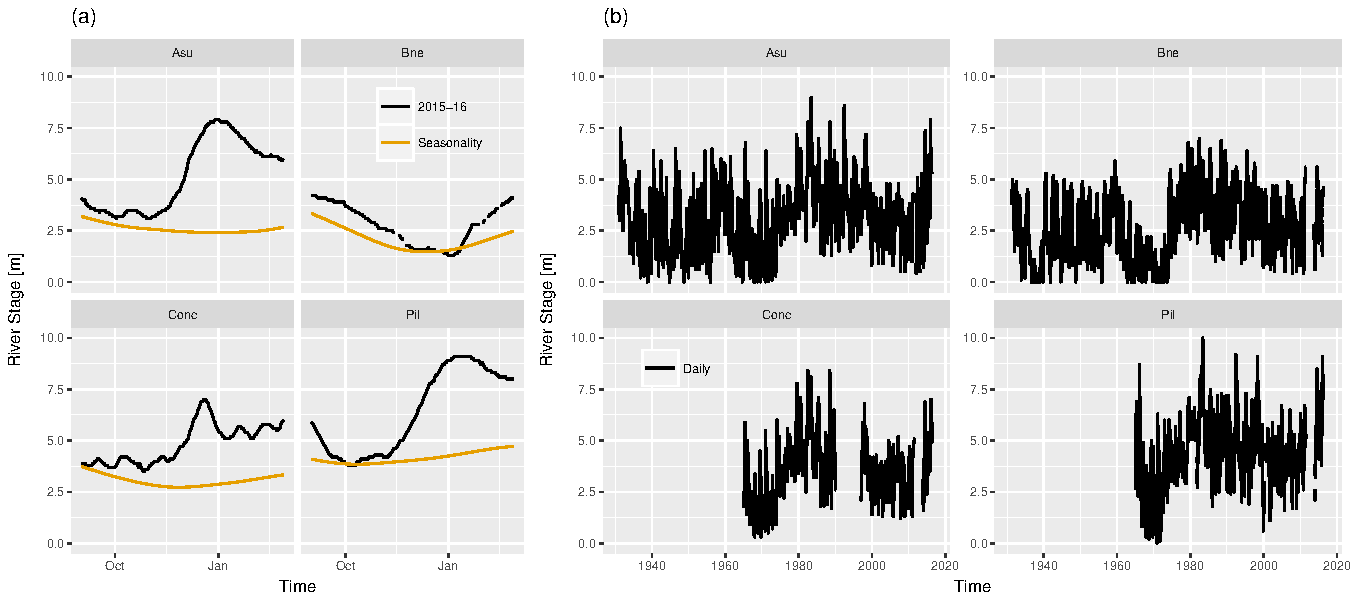
\includegraphics[width=6.5in]{./Streamflow.pdf}
	\caption{
		River stage (height; in \si{\meter}) for the Paraguay River at four gauges along the Paraguay River.
		(a) Seasonality (orange) and time series of 2015-16 observations (black) at each stream gauge.
			The seasonality was fit using local polynomial regression as implemented in the \texttt{locfit} package in
			the \textbf{R} statistical programming environment \citep{Loader1999}.
		(b) Time series of daily stage measurements from 1929 to 2016 at each station.
	}
  \label{fig:streamflow}
\end{figure*}

\begin{figure*}
	\noindent\includegraphics[width=6.5in]{../_figs/NDJF201516Anomaly.pdf}
	\caption{
    	Monthly composite anomalies observed during NDJF 2015-16.
      Top row shows anomalies of streamfunction $\psi$ at \SI{850}{\hecto\pascal}.
      Bottom row shows monthly rainfall anomalies, in units of \si{\milli\meter\per\day}.
	}
  \label{fig:anomalies}
\end{figure*}

\begin{figure*}
	\noindent\includegraphics[width=6.5in]{../_figs/PSI_EOF_Loadings.pdf}
	\caption{
    	Leading four EOF loadings of daily NDJF \SI{850}{\hecto\pascal} streamfunction $\psi$ over chosen domain.
	}
  \label{fig:eof-loading}
\end{figure*}

\begin{figure*}
	\noindent\includegraphics[width=6.5in,height=9in,keepaspectratio=true]{../_figs/WTComposite.pdf}
	\caption{
		Composite anomalies associated with each weather type (column).
    Top row shows anomalies of streamfunction $\psi$ at \SI{850}{\hecto\pascal}.
    Bottom row shows precipitation anomalies in units of \si{\milli\meter\per\day}.
	}
	\label{fig:wt-composite}
\end{figure*}

\begin{figure*}
	\noindent\includegraphics[width=6.5in]{../_figs/RainfallWeatherType}
	\caption{
		Time series of area-averaged rainfall in the Lower Paraguay River Basin (\cref{fig:study-area}) for each day of NDJF  2015-16 (lines).
		The weather types corresponding to each day are indicated in both color and adjacent label.
		Dashed lines indicate the climatological 50th, 90th, and 99th percentiles of NDJF area-averaged rain over the Lower Paragauy River basin.
	}
  \label{fig:rain-wt}
\end{figure*}

\begin{figure*}	\noindent\includegraphics[width=6.5in]{../_figs/LaggedRain.pdf}
	\caption{
		Circulation anomalies associated with intense rainfall (99th percentile exceedance of area-averaged rainfall in the Lower Paraguay River Basin shown in \cref{fig:study-area}).
		Lagged composites are shown, by column, for $t = $ \SIlist{-2;-1;0;1}{\day} relative to the date of intense rainfall.
		Top row shows anomalies of streamfunction $\psi$ at \SI{850}{\hecto\pascal}.
    Bottom row shows precipitation anomalies in units of \si{\milli\meter\per\day}.
	}
  \label{fig:lagged-rain}
\end{figure*}

\begin{figure*}
	\noindent\includegraphics[width=6.5in]{../_figs/Chiclet.pdf}
	\caption{
    S2S model forecasts of area-averaged rainfall over the Lower Paraguay River Basin (\cref{fig:study-area}).
    Forecast time series from the ECMWF S2S model are shown for several lead times (\SIlist{5;14;19;30}{\day}).
		Each gray dot represents the forecast of a single ensemble member issued for the target date ($x$-axis) of area-averaged rainfall, in \si{\milli\meter\per\day} ($y$-axis).
		The blue line connects the ensemble means, and the black line shows the observed rainfall.
		Because the model is initialized twice-weekly, for a given lead time forecasts will only exist for two in seven possible target dates;  consequently the rainfall is smoothed with a 3-day running mean to facilitate visual comparison.
	}
  \label{fig:chiclet}
\end{figure*}

\begin{figure*}
	\noindent\includegraphics[width=6.4in]{../_figs/ForecastSkill.pdf}
	\caption{
		MOS-adjusted S2S model forecasts and skill scores for the methods indicated in \cref{tab:mos-methods}.
		Top row shows the intense rainfall forecast for 1-7 December 2015 as the odds ratio of \cref{eq:odds-ratio} over the target domain.
		A value greater than 1 indicates that the model forecast greater-than-average odds of rainfall exceeding the 90th percentile.
		The second shows the 2AFC skill score for each grid cell; a value greater than 50 indicates that the model outperforms climatology.
	}
  \label{fig:subs-prob-fcst}
\end{figure*}

\begin{figure*}
	\noindent\includegraphics[width=6.5in]{../_figs/SeasonalForecast.pdf}
	\caption{
	Seasonal model forecast.
	Shading indicates the forecast probability of exceeding the 90th percentile of climatological rainfall during DJF 2015-16.
	As \cref{fig:subs-prob-fcst}, the variable shown is the odds ratio of \cref{eq:odds-ratio} over the target domain.
	A value greater than 1 indicates that the model forecast greater-than-average odds of rainfall exceeding the 90th percentile.
	}
  \label{fig:seas-prob-fcst}
\end{figure*}

\end{document}
